\subsection{Open set, closed set, neighborhood}


\begin{exercise}{1}
Justify the terms ``open ball'' and ``closed ball'' by proving that (a) any open ball is an open set, (b) any closed ball is a closed set.
\end{exercise}
\begin{proof}
(a) This follows the same logic as in the converse of exercise 4.

(b) Consider the closed ball with radius $r$ around $x$, $B=B(x;r)$. Let $y\in B^C$, and $r'=\min[d(y,x+r), d(y,x-r)]$, we have that $B(y;r'/2)\subseteq B^C$, so that for any point in $B^C$ there is an open ball containing it, that is, $B^C$ is open and thus $B$ is closed.
\end{proof}

\begin{exercise}{2}
What is an open ball $B(x_0; 1)$ on $\R$? In $\C$ (Cf. 1.1-5)?  In $C[a,b]$ (Cf. 1.1-7)? Explain the following figure.
\begin{figure}[H]
    \centering
    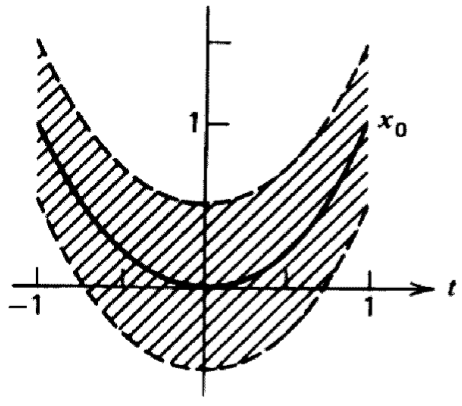
\includegraphics[width=0.5\textwidth]{kreyszig/assets/sec1-3-ex2.png}
    \caption{Region containing the graphs of all $x\in C[-1,1]$ which constitute the $\epsilon$-neighborhood, with $\epsilon=1/2$, of $x_0\in C[-1,1]$ given by $x_0(t)=t^2$.}
    \label{fig:fig1-3}
\end{figure}
\end{exercise}
\begin{proof}
$\R$: An open interval of the form $(a,b)$, where $b-a=2$ and the midpoint is $x_0$.

$\C$: If we think of $\C$ as $\R^2$ then it is a circle centered at $x_0$ with radius $1$, without the circumference of the circle.

$C[a,b]$: All the functions $g$ so that $\absoluteValue{g(t)-x_0(t)}<1$ for all $t$. 

We can see something similar in \Cref{fig:fig1-3}, where the shaded area is the area where the functions with $\absoluteValue{g(t)-t^2}<1/2$ can go through, for $t\in[-1,1]$.
\end{proof}

\begin{exercise}{3}
Consider $C[0,2\pi]$ and determine the smallest $r$ such that $g\in \hat{B}(f;r)$, where $f(t)=\sin t$ and $g(t)=\cos t$.
\end{exercise}
\begin{proof}
$r=1$ suffices, since the largest difference between $\sin t$ and $\cos t$ is 1 whenever $t=0$.
\end{proof}

\begin{exercise}{4}
Show that any nonempty set $A\subseteq (X,d)$ is open if and only if it is a union of open balls.
\end{exercise}
\begin{proof}
($\Rightarrow$) Suppose $A$ is open, then for every point in $x$ there is an open ball which is a subset of $A$. Thus $A$ is composed of open balls. That is, $A$ is a union of open balls.

($\Leftarrow$) Suppose $A$ is a union of open balls. Then any point in $x\in A$ belongs to one of these open balls, say $B(y;r)$. Let $r'=\min[d(x,y+r), d(x,y-r)]$, then $B(x;r')\subseteq B(y;r)\subseteq A$, so that there is an open ball around $x$ and $A$ is open.
\end{proof}

\begin{exercise}{5}
It is important to realise that certain sets may be open and closed at the same time. (a) Show that this is always the case for $X$ and $\emptyset$. (b) Show that in a discrete metric space $X$ (Cf. 1.1-8), every subset is open and closed.
\end{exercise}
\begin{proof}
(a) On page 19 Kreyszig proved that $\emptyset$ and $X$ are open. A set is closed if its complement is open. Hence given $X^C=\emptyset$ and $\emptyset^C=X$, both $X$ and $\emptyset$ are closed.

(b) From (a) we know that $X$ and $\emptyset$ are open and closed so let's consider a non trivial subset of $X$. Notice that every nonempty subset of $X$ is open, because for any $x\in X$, the set $\set{x}$ is a ball $B(x; r)$ for any $r<1$. But this means that the complement of any nonempty subset of $X$ is open because the same holds for any element of $X$. Hence, all subsets of $X$ are open and closed (clopen).
\end{proof}

\begin{exercise}{7}
Describe the closure of each of the following subsets. (a) The integers on $\R$, (b) the rational numbers on $\R$, (c) the complex numbers with rational real and imaginary parts in $\C$, (d) the disk $\set{z: \absoluteValue{z}<1}\subseteq\C$.
\end{exercise}
\begin{proof}
(a) Let $x\in\R$ and $x\notin\Z$. Notice that there are two integers $a,b$ so that $a<x<b$. Let $r=\min[x-a, b-x]$. We then have that $B(x,r)$ does not contain any element of $\Z$ and thus $x$ is not an accumulation point of $\Z$ in $\R$. As a result, $\Z=\overline{\Z}$ in $\R$.

(b) By the density of the rationals in the reals, any open ball around a rational contains an irrational number and hence it is an accumulation point. As a result, $\overline{\Q}=\R$.

(c) Following the same logic of (b), the closure of the complex numbers with rational real and imaginary parts is $\C$.

(d) This is similar to (b) and (c). Simply let $x\in\C$ have $\absoluteValue{x}=1$. For any $\epsilon>0$ we will always find that the ball $B(x;\epsilon)$ will contain an element of $\set{z: \absoluteValue{z}<1}$, so that $x\in\overline{\set{z: \absoluteValue{z}<1}}$. On the other hand, any number $y\in\C$ with $\absoluteValue{y}>1$ has an $\epsilon$-neighborhood so that no element of $\set{z: \absoluteValue{z}<1}$ belongs to it. Putting this together, we conclude that $\overline{\set{z: \absoluteValue{z}<1}}=\set{z: \absoluteValue{z}\leq 1}$.
\end{proof}

\begin{exercise}{8}
Show that the closure $\overline{B(x_0;r)}$ of an open ball $B(x_0;r)$ in a metric space can differ from the closed ball $\hat{B}(x_0;r)$.
\end{exercise}
\begin{proof}
Consider a set $X$ with the discrete metric. We have that $\hat{B}(x,1)=X$ for any $x\in X$. However, let $x,y\in X$ and consider the open ball $B(x;1)=\set{x}$. Think of the $\epsilon$-neighborhood around $y$ with $\epsilon=1/2$. Such $\epsilon$-neighborhood does not contain any element of $B(x;1)$, and so $y$ is not an accumulation point of $B(x;1)$. As a result, $B(x;1)=\overline{B(x;1)}\neq\hat{B}(x,1)=X$, as required.
\end{proof}

\begin{exercise}{9}
Show that 
\begin{enumerate}
    \item $A\subseteq\overline{A}$.
    \item $\overline{\overline{A}}=\overline{A}$.
    \item $\overline{A\cup B}=\overline{A}\cup\overline{B}$.
    \item $\overline{A\cap B}\subseteq\overline{A}\cap\overline{B}$.
\end{enumerate}
\end{exercise}
\begin{proof}
\begin{enumerate}
    \item By definition $\overline{A}$ contains $A$.
    \item We will prove this by double containment. $\overline{\overline{A}}\supseteq\overline{A}$ follows directly from the definition of closure. For the other direction, let $x\in \overline{\overline{A}}$. Then $x$ is either:
    
    (i) In $\overline{A}$, in which case $x\in\overline{\overline{A}}$ or,
    
    (ii) $x$ is an accumulation point of $\overline{A}$ not in $\overline{A}$.
    
    So suppose $x\notin \overline{A}$. Fix $\epsilon>0$, because $x$ is an accumulation point, there exists $y\in\overline{A}$ such that $d(x,y)\leq \epsilon/2$, and likewise because $y$ is in $A$ or it is one of its accumulation points, then  there exists $z\in A$ such that $d(y,z)\leq \epsilon/2$. Hence, $d(x,z)\leq d(x,y)+d(y,z) =\epsilon$ and so $x$ is an accumulation point of $A$ resulting in $x\in\overline{A}$. This contradicts (ii) so it must be the case that $x\in\overline{\overline{A}}$.
    \item We will prove this by double containment. 

    ($\subseteq$) Let $x\in\overline{A}\cup\overline{B}$. Then $x$ is either in $A$ or $B$ or an accumulation of either. If $x\in A$ or $x\in B$, then $x\in\overline{A}\cup\overline{B}$, so suppose $x\notin A,B$. Without loss of generality, suppose $x$ is an accumulation point of $A$. Then for every $\epsilon>0$, an open ball centered around $x$ with radius $\epsilon$ contains an element of $A$. But certainly it contains an element of $A\cup B$, so that $x\in\overline{A\cup B}$.

    ($\supseteq$) Let $x\in\overline{A\cup B}$. Then either $x\in A\cup B$ or $x$ is an accumulation of the union. In the former case, we would have that $x\in\overline{A}$ or $x\in\overline{B}$, so suppose that's not the case. Since $x$ is an accumulation point of $A\cup B$, then it must be the case there are infinite elements of $A\cup B$ that intersect open balls centered at $x$ (suppose this wasn't the case, then we could take the minimum of the distances between $x$ and every one of those elements of $A\cup B$, and then the open ball centered at $x$ with half such distance would not contain any element of $A\cup B$). However, this implies that there are either infinite elements of $A$ or infinite elements of $B$ that intersect open balls centered around $x$ (of any arbitrarily small radius), so that either $x\in\overline{A}$ or $x\in\overline{B}$.
    \item Suppose $x\in\overline{A\cap B}$, then either $x\in A\cap B$ or $x$ is an accumulation point of such set. If $x\in A\cap B$, then $x\in A$ and $x\in B$ so certainly $x\in\overline{A}\cap\overline{B}$ since $A\subseteq\overline{A}$ and $B\subseteq\overline{B}$. So suppose $x$ is an accumulation point of $A\cap B$. This implies that for every $\epsilon>0$, the open ball of radius $\epsilon$ centered at $x$ contains an element $y\in A\cap B$. Thus, for every $\epsilon>0$, there exists an element of $A$ such that it belongs to the open ball centered around $x$, so that $x\in\overline{A}$, following the same argument we can conclude that $x\in\overline{B}$ as well. That is, $x\in\overline{A}\cap\overline{B}$.
    \end{enumerate}
\end{proof}

\begin{exercise}{11 (Boundary)}
A boundary point $x$ of a set $A\subseteq (X,d)$ is a point of $X$ (which may or may not belong to $A$) such that every neighborhood of $x$ contains points of $A$ as well as points not belonging to $A$; and the boundary (or frontier) of $A$ is the set of all boundary points of $A$. Describe the boundary of (a) the intervals $(-1,1), [-1,1), [-1,1]$ on $\R$; (b) the set of all rational numbers on $\R$; (c) the disks $\set{z:\absoluteValue{z}<1}\subseteq\C$ and $\set{z:\absoluteValue{z}\leq 1}\subseteq\C$.
\end{exercise}
\begin{proof}
(a) For all intervals $-1$ and 1 are the boundary points. Simply consider for any $\epsilon>0$ the open ball around any of these two points. We will obtain than points in the intervals (and outside of them), are in such ball.

(b) Since the rationals are dense in $\R$, any open ball around any rational will contain both rationals and irrationals. Furthermore, for any irrational, we can find a rational that gets arbitrarily close to it. Hence, $\R$ is the boundary of $\R$.

(c) In both cases, the set $\set{z:\absoluteValue{z}=1}\subseteq\C$ is the boundary of the disks. That is because for any open ball around these points, we can find elements withing the disks and outside of them.
\end{proof}

\begin{exercise}{12 (Space $B[a,b]$)}
 Show that $B[a,b]$, $a<b$ is not separable (Cf. 1.2-2).
\end{exercise}
\begin{proof}
Suppose, for the sake of contradiction, that $B[a,b]$ is separable. Then there exists a countable set, call it $\FFF$, of functions so that for all functions in $g\in B[a,b]$, either $g\in\FFF$, or for all $\epsilon>0$, there exists a function $f\in\FFF$ with $f\in B(g;\epsilon)$.

Since $\FFF$ is countable we can find a bijection between $\FFF$ and $\N$, so that we can have a sequence of distinct numbers, $(x_n)$ where each $x_i\in[a,b]$ and $x_n$ can be mapped to a function, say $f_n\in\FFF$. Now let $h\in B[a,b]$ be defined as follows: for $h(x_n)=f_n(x_n)+1$ and 0 otherwise. We have that the open ball $B(h;1/2)$ does not contain any element of $\FFF$, so that $h$ is not an accumulation point of $\FFF$. Thus, $\overline{\FFF}\neq B[a,b]$ and $B[a,b]$ is not separable. 
\end{proof}

\begin{exercise}{13}
Show that a metric space $X$ is separable if and only if $X$ has a countable subset $Y$ with the following property. For every $\epsilon>0$ and every $x\in X$ there is a $y\in Y$ such that $d(x,y)<\epsilon$.
\end{exercise}
\begin{proof}
($\Rightarrow$) Suppose $X$ is separable. Then there exists a countable subset $Y\subseteq X$ so that $\overline{Y}=X$. But this means that for every $x\in X$, either $x\in Y$ or that for all $\epsilon>0$, there exists a $y\in Y$ with $y\in B(x, \epsilon)=\set{z\in X:d(x,z)<\epsilon}$, giving us the desired result.

($\Leftarrow$) Suppose there exists a countable subset $Y\subseteq X$ so that for every $\epsilon>0$, and every $x\in X$, there exists a $y\in Y$ with $d(x,y)<\epsilon$. Then this means that every $x\in X$ is an accumulation point, because for every $x$ and $\epsilon>0$ we can find $y\in Y$ with $y\in B(x,\epsilon)$. However, since all $x\in X$ are accumulation points of $Y$, then $\overline{Y}=X$, giving us that $X$ is separable, as required.
\end{proof}

\begin{exercise}{14 (Continuous mapping)} Show that a mapping $T:X\to Y$ is continuous if and only if the inverse image of any closed set $M\subseteq Y$ is a closed set in $X$.
\end{exercise}
\begin{proof}
Let $M$ be closed so that $M^C$ is open. By definition, we have that $(T^{-1}(M))^C=\set{x\in X:T(x)\notin M}=T^{-1}(M^C)$. 

For the ($\Rightarrow$) proof, if $T$ is continuous, then the inverse image of an open set is open, so that $T^{-1}(M^C)$ is open and by the equality above, then the inverse image of a closed set is closed. That is, $(T^{-1}(M))^C$ is open. 

For the converse, $(\Leftarrow)$, if the inverse image of a closed set is closed, so that $(T^{-1}(M))^C$ is open, by the equality above, we get that $T^{-1}(M^C)$ is open, so that the inverse image of an open set is open. That is, $T$ is continuous.
\end{proof}

\begin{exercise}{15}
Show that the image of an open set under a continuous mapping need not be open.
\end{exercise}
\begin{proof}
We have that $f:\R\to\R$ given by $f(x)=x^2$ is continuous. Consider the open set $A=(-1,1)\in\R$. We have that $f(A)=[0,1)$, which is not open in $\R$ because there is no open ball around 0 fully contained in $[0,1)$.
\end{proof}
